\documentclass[a4paper,10pt]{article}
\usepackage[utf8]{inputenc}
\usepackage{textcomp} % Degree symbol
\usepackage{xcolor} % Grey comments
\usepackage[colorlinks, allcolors=blue]{hyperref}
\usepackage{graphicx}
\usepackage{pgfgantt} % Gantt chart
\usepackage{natbib}
\bibliographystyle{apalike}

%opening
\title{Fuzzy land cover classification method assessment using PROBA-V satellite data}
\author{Dainius Masili\=unas}

\begin{document}

\maketitle

\section{Introduction}

Global land cover mapping is very important from an ecological and earth systems point of view. Land cover maps are used for a variety of applications, from estimating area covered by forests \citep{bartalev2014probavboreal} to air quality modelling \citep{wiedinmyer2006airquality}. In addition, land cover maps, especially those of fine spatial resolution, have the potential to be used for land cover change monitoring \citep{defourny2012cci}. This is important for a number of land cover classes. For instance, forests are an important terrestrial carbon sink in the global carbon cycle, with different forests having different carbon sink capacities \citep{pan2011large}. Knowing their distribution and changes over time allows for more accurate climate change modelling. Another land cover class, wetlands, is key for maintaining biodiversity due to the uniqueness of wetland ecosystems that allows rare and protected species to live there. Wetlands are protected globally by the Ramsar convention \citep{davis1994ramsar}.

The creation of a global land cover map from remote sensing data has been a goal of many different studies \citep{hansen2000hardtree}. Their results are nowadays freely available as satellite imagery products, such as Global Land Cover 2000 \citep{bartholome2005glc2000}, MODIS land cover \citep{friedl2010modis} and GlobCover \citep{arino2007globcover}. There are also maps based on the fusion of multiple other maps, like Geo-Wiki hybrid \citep{see2015hybrid}, and multiple sensors, like Land Cover CCI \citep{lccciguide} and GlobeLand30 \citep{chen2015globeland30}. However, these land cover maps all have certain drawbacks.

The first common drawback of current global land cover classification products is that their spatial resolution is low to medium. The majority of aforementioned land cover products are derived from MODIS and MERIS sensor data. The sensors are only capable of capturing images with the finest pixels representing 300 by 300 metre areas (at the equator). Recent advances in satellite sensors and computing power would allow for land cover classification at a higher spatial and temporal resolution. For example, at the moment the PROBA-V mission by the European Space Agency produces imagery that is a good fit for use in land cover classification. It has spatial resolution as fine as 100 by 100 metre pixels (with additional products also providing 300 by 300 metre and 1 by 1 kilometre pixel size for comparison with previous sensors) \citep{probavguide}. It is well-suited for time series analysis, because it has an archive that goes back to 2013, as well as a fast revisit time of 2 days for full global coverage (1 day for locations above 35\textdegree{} latitude) \citep{dierckx2014probav}.

The second drawback of current global land cover products is that their classification accuracy tends to be low, averaging at around 65\% \citep{tsendbazar2016integrating}. The third drawback is that all of these products use what is known as ``hard'' or ``crisp'' classification: each pixel on the map is made to represent only one land cover type.

Hard classification is not well-suited for coarse resolution imagery, due to a large proportion of mixed pixels in it, compared to endmember (pure) pixels. When hard classification is attempted on such imagery, the accuracy of the result can be no higher than the area fraction that the dominant land cover type of the pixel occupies \citep{latifovic2004accuracy}. There have been attempts at increasing accuracy by defining mosaic classes, such as mixed forests (50\% needleleaf and 50\% broadleaf trees), but it leads to a proliferation of classes that increases map complexity and still does not deal with the core problem, thus not improving the classification accuracy by much \citep{tsendbazar2016comparative}. In contrast, ``fuzzy'' or ``soft'' classification results in each pixel containing information about the fraction of each class within that pixel, therefore operating on sub-pixel scales. This has the advantage of representing land cover more accurately, and gives the ability to represent mosaic classes as a combination of pure classes instead. Since the output of fuzzy classification is essentially one raster per class, with smooth edges, it is suitable for more in-depth analysis and user-specific visualisation criteria \citep{tsendbazar2016integrating}. Despite that, hard classification is still the most often used classification type due to the number of algorithms developed for it, ease of storing the result (it is thematic and thus takes little storage space), displaying it in a single map (albeit in a less accurate fashion) and performing accuracy assessment.

There is a number of different classification algorithms, but only several of them are suitable to be used for fuzzy classification \citep{nath2014methods}. The two methods most commonly used in scientific literature are fuzzy c-means and neural networks \citep{zhang2001fullyfuzzy}. Neural networks in particular are well-suited for fuzzy classification, since they allow multiple continuous output as well as input variables in a single model \citep{foody1997fuzzynnet}. Fuzzy c-means, also known as fuzzy k-means or soft k-means, is a statistical method that relies on the proximity of pixels in feature space to class centroids, and thus is also suitable for fully fuzzy classification. However, since k-means is an unsupervised classification algorithm, the ability to make use of training data in fuzzy c-means is limited to determining class centroids with more precision \citep{hengl2004fuzzycmeans}, and as such it is effectively similar to maximum likelihood classification.

In addition, any other algorithms that provide a measure of uncertainty about class membership can be used, such as the ratio of individual tree votes of random forest \citep{breiman2001random} or class probabilities in gradient boosting \citep{friedman2001gradientboost}. While classification uncertainty is not a direct measure of class membership \citep{sytze2000fuzzyset}, they are nonetheless correlated. As such, it has been used by numerous authors as a proxy indicator of class membership, achieving satisfactory classification accuracy \citep{foody2002accuracy}.

Furthermore, algorithms that can handle continuous variables, but only one response variable (such as random forest), can be used as well, by creating separate models for every class. This approach is called Binary Relevance \citep{karalas2016br}. Using this approach, the data needs to be post-processed after classification at a pixel level to conform to physical constraints (class membership must be between 0 and 100\% and sum up to 100\%). Random forest has been reported to give higher or equal accuracy results compared to other algorithms, like Support Vector Machines and individual decision trees, in hard classification scenarios using satellite imagery similar to that of PROBA-V \citep{duro2012algorithmcomparison}. Random forest regression was also shown to perform as well as other algorithms in fuzzy classification scenarios \citep{walton2008subpixelrf}, although it is used in much fewer studies on fuzzy classification than the other algorithms mentioned previously. Gradient boosting is an algorithm related to random forest, with the same advantages and disadvantages, but it is known to perform better in machine learning challenges \citep{chen2015higgs} and has not yet been tested on fuzzy land cover classification.

Accuracy assessment is rather straight-forward for hard classification: typically a confusion matrix is employed for this purpose, showing how many pixels (or in some cases how much area \citep{stehman2009sampling}) in the image have been classified correctly, and how many incorrectly. Such a matrix makes it simple to tell which classes are hard to discern from one another, as well as allows for deriving statistics such as users' accuracy, producers' accuracy, and total accuracy \citep{foody1996fuzzyevaluation}, as well as variance if probability sampling was used. However, a standard confusion matrix is not applicable in the context of fuzzy classification, since misclassification in this case is not absolute, but rather a matter of degree \citep{foody2002accuracy}. Several solutions, such as distance \citep{foody1996fuzzyevaluation}, cross-entropy and mutual information \citep{lu2007methods} have been suggested as alternatives for fuzzy classification accuracy assessment.

Visualisation of the fuzzy classification results is also challenging, since each class effectively is a single-channel raster of its own. Three such classes can easily be combined into RGB channels for visualisation, but with more classes it is no longer possible. There have been attempts to develop a method based on the hue, saturation and intensity colour model to allow for a larger number of distinct classes to be visualised on a single raster \citep{hengl2004fuzzycmeans}. There is also a possibility of ``hardening'' the classification when high accuracy visualisation is not needed, and making use of multiple RGB rasters side-by-side when it is needed.

All in all, even though global land cover mapping has been a focus of many other studies, existing global land cover maps still have room for improvement. This can be achieved by using data from the sensors of newer satellites such as PROBA-V, as well as performing fuzzy classification as opposed to the traditional hard classification.

\section{Problem definition and research questions}

An important long-term goal of land cover mapping is to have a highly accurate fuzzy land cover classification method at a global scale. Since there are many different methods that could be used to achieve such a goal, and since the amount of data generated by satellites covering the entire world is enormous, this thesis will focus on comparing several different fuzzy classification algorithms on a subset of global imagery provided by the PROBA-V satellite.

PROBA-V is a relatively new satellite, with few studies using it for land cover classification so far. A number of studies have used simulated PROBA-V data in preparation for its launch \citep{stathakis2014probavurban,roumenina2013probavcrops,bartalev2014probavboreal}. After launch, most studies have focused on its potential for crop classification \citep{roumenina2015probavcrops,durgun2016crop,lambert2016cropland}. All of these studies have only used the traditional hard classification. As such, the potential of using fuzzy classification to obtain a more accurate representation of land cover at global scale has never been tested before.

In addition, this study will focus specifically on the region of ecotone from boreal forests to temperate broadleaf forests in Europe. This region also includes a large number of boreal wetlands. Both mixed forests and wetlands are challenging to detect and classify using traditional remote sensing techniques, thus it is important to check how well large scale fuzzy classification performs on these classes.

There is a wide variety of algorithms that can be used for fuzzy classification. In this thesis, four of them will be tested: fuzzy c-means, neural networks, random forest regression and multiclass gradient boosting. All of these algorithms are based on fundamentally different approaches to classification, so the results will give insight into the possible performance of similar algorithms as well. In addition, the last of the mentioned algorithms has not yet been tested on fuzzy classification itself (although related algorithms have been).

The accuracy of classification results is not the only relevant difference between the algorithms. Another important aspect to consider is the processing time. It is especially important for global image processing, which is firmly in the realm of big data. Some algorithms are known to suffer from the curse of dimensionality, where a linear increase in input data results in a geometric increase in processing time \citep{walton2008subpixelrf}.

In addition to algorithms, one aspect that is important for classification accuracy is the data (training variables) that the algorithm is trained on \citep{yu2014metadiscoveries}. In addition to spectral variables (blue, red, near infrared, shortwave infrared bands), temporal variables (growing season start, duration, growing intensity) are commonly used to improve the separability of crops \citep{jakubauskas2001harmonic}. Elevation variables (elevation, slope, aspect) are known to improve the separability between tree classes \citep{burrough2001fuzzy}. Vegetation indices have been used to improve the detection of wetlands \citep{sader1995wetlands}, as well as for defining classification rules in rule-based fuzzy classfication \citep{baraldi2006rulebased}. Therefore in this thesis such variables will also be used in order to increase land cover classification accuracy.

Thus the goal of this thesis is to improve large-scale land cover maps by performing fuzzy land cover classification in the boreal forest-temperate broadleaf forest gradient zone using PROBA-V satellite imagery. The research questions that the thesis will attempt to answer are:

\begin{itemize}
 \item Which fuzzy classification algorithm (fuzzy c-means, neural networks, random forest regression, multiclass gradient boosting) gives the highest per-class and total classification accuracies?
 \item How much does the classification accuracy change when more variables are added to classification models? Which variables are most important for classification?
 \item What is the difference in processing speed between the different algorithms, when subjected to increasing amounts of data to process?
\end{itemize}

\section{Methods}

\subsection{Input data}

The PROBA-V image that will be used to derive spectral data for classification will be selected from the ones available based on these criteria: the date of acquisition has to be during the summer of 2016, since that minimises the effects of snow and senescence \citep{bartalev2014probavboreal}; the number of good-quality pixels (not affected by clouds, sensor problems, etc.) in the tile should be as high as possible; and the spatial resolution of the image should be as fine as possible (ideally 100 m resolution). Composites of several days will be used to get higher quality images. Images closer to the present will be preferred if there are several images that match the previous criteria (i.e. their quality is equal).

For deriving temporal data (vegetation growth phase, amplitude and period), a series of images spanning the entire lifetime of the PROBA-V mission (2013-2016, 3 years) will be used. The variables will be extracted by performing harmonic analysis \citep{rayner1971introduction,jakubauskas2001harmonic} on NDVI time series of the imagery.

\begin{figure}
 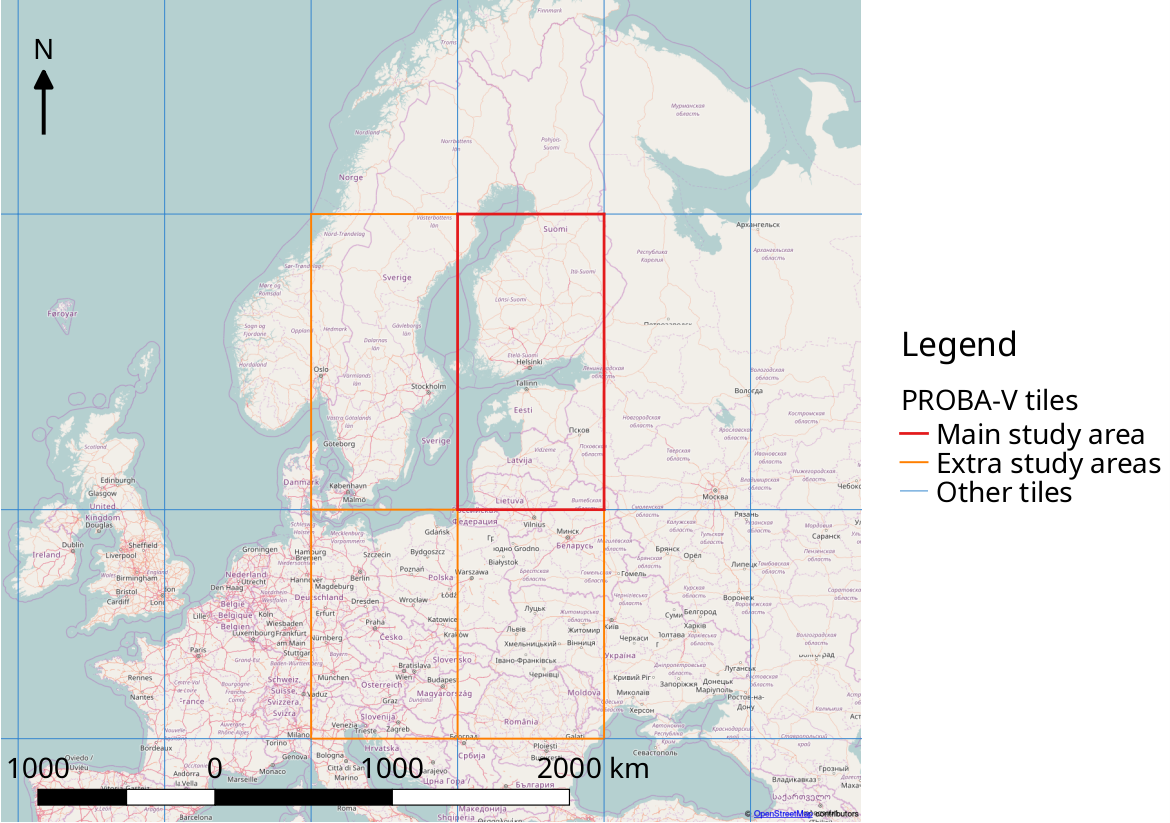
\includegraphics[width=\textwidth]{./proposal-figures/studyarea.png}
 \caption{Study area. The grid represents PROBA-V tiles (10 by 10 degree areas), tile 20,01 is highlighted in red, tiles 20,02, 19,01 and 19,02 are highlighted in orange.}
 \label{AOI}
\end{figure} 

The study area will be based on the PROBA-V tile 20,01. It spans from south Finland, known for boreal forests as well as a variety of lakes and boreal wetlands, to the middle of Lithuania, which includes both mixed and temperate broadleaf forests as well as protected wetlands. If time permits, tiles 20,02 (from middle of Lithuania to north of Bulgaria), 19,01 (south Sweden) and 19,02 (from north Poland and Germany to north Italy and Croatia) will also be used, by mosaicing them all into one large image (see figure \ref{AOI}).

In addition to that, auxiliary variables will be used in classification. In particular, the digital elevation model (DEM) from the NASA Global Land Survey will be used to derive elevation, slope and aspect terrain parameters. These parameters are known to increase the separability of vegetation classes \citep{burrough2001fuzzy}, and this particular DEM is already used by PROBA-V product suppliers for image ortho-rectification \citep{probavguide}.

A variety of vegetation indices are known to improve the separability of the wetlands class \citep{zhao2009indices,davranche2010wetland}. However, since the PROBA-V sensor only captures four spectral bands, the choice of available vegetation indices is limited. Therefore two vegetation indices that can be calculated and are known to improve wetlands separability will be used: Optimised Soil-Adjusted Vegetation Index (OSAVI) and Land Surface Water Index (LSWI). While there is a possibility of using data from other sensors for deriving vegetation indices, attempting to match their pixels to those of PROBA-V is bound to introduce inaccuracies due to resampling, thus that will not be attempted.

\subsection{Classes}

The land cover classes that will be used for classification are based on the hybrid classification scheme by \citep{see2015hybrid}. The only change is the distinction between evergreen and deciduous tree cover (defined by whether the leaves have an annual senescence cycle or not):
\begin{enumerate}
 \item Deciduous trees
 \item Evergreen trees
 \item Shrubs
 \item Grassland
 \item Cropland
 \item Wetland
 \item Urban
 \item Permanent snow or ice
 \item Bare soil
 \item Water
\end{enumerate}

\subsection{Collection of training and validation data}

Samples for training and validation will be obtained manually, by following a procedure adapted from \citep{defries1998training}:
\begin{itemize}
 \item The chosen PROBA-V raster tile will be imported into QGIS as a boundary reference. From it, a line grid will be created to serve as a boundary reference for every pixel of the original image.
 \item The latest LC-CCI dataset will be imported into QGIS in order to serve as a basis for land cover stratification. The raster will be converted to polygons and classes will be merged to conform to the classes listed in the previous section.
 \item A new point layer for determined class fractions will be created.
 \item Other layers, like OpenStreetMap, Google Satellite (e.g. Digital Globe), Bing Maps, SENTINEL-2 imagery, and aerial photography, will be put on top of the PROBA-V raster tile. When there is an option, reference data closest to the date of the image to be classified will be preferred.
 \item 1000 points will be generated using stratified random sampling within the boundaries of the PROBA-V raster tile. Merged LC-CCI land cover types will be used as strata. Each pixel that the points fall onto will be selected as a potential pixel to be used for class fraction determination.
 \item Each selected pixel will have its land cover class fractions filled out (one attribute per class, summing up to 100\%). These fractions will be determined using visual inspection and interpretation of all the aforementioned layers. To maximise the accuracy in mixed pixels, the fractions will be calculated by measuring the area each class occupies within the pixel, then dividing it by the total area the pixel occupies. See figure \ref{fig-procedure} for an example.
 \item The process will be repeated until each class has a representative sample of pixels classified (a minimum of 50 pixels per class and 15 endmember pixels among them).
\end{itemize}

Some of the randomly generated points may be skipped, if it is unclear from the reference data which classes the pixel contains. After 50 pixels have been classified, and there are fewer than 15 endmember pixels of a particular class among the pixels classified, some mixed pixels may also be skipped. A large enough sample of endmember pixels is important for training algorithms that do not allow training on mixed pixels.

The resulting sample points will then be imported into R. Each attribute in R is available as a variable, so they can then be used in classification.

\begin{figure}
 \centering
 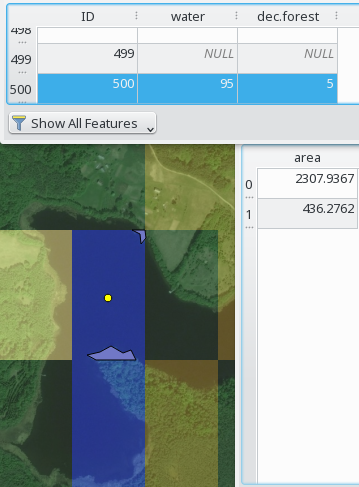
\includegraphics[width=7cm]{./proposal-figures/procedureexample.png}
 \caption{An example of a validated pixel (centre). The non-dominant land cover class (deciduous trees) fraction has been determined by placing polygons over it, calculating the area (right), dividing it by the total area in the pixel and filling out the information in the attribute table of the point in the centre of the pixel (top).}
 \label{fig-procedure}
\end{figure}

\subsection{Classification algorithms}

There will be four classification algorithms tested in total: fuzzy c-means, fuzzy neural network, random forest regression and multiclass gradient boosting. All of these algorithms are available as pacakges for the \texttt{R} programming language. See table \ref{tbl-comparison} for a short comparison of the properties of the chosen algorithms.

\begin{table}
  \begin{center}
    \resizebox{\textwidth}{!}{
      \begin{tabular}{lllll}
	\hline
	Algorithm name & Supervised? & Fuzzy? & Single-model? & Type\\
	\hline
	Fuzzy c-means & Partially & Yes & Yes & Statistical\\
	Fuzzy neural network & Yes & Yes & Yes & Machine learning\\
	Random forest regression & Yes & Yes & No & Machine learning\\
	Multiclass gradient boosting & Yes & Partially & Yes & Machine learning\\
	\hline
      \end{tabular}
    }
  \end{center}
  \caption{Feature comparison between classification algorithms whose classification accuracy will be compared in the thesis. ``Partially fuzzy'' means the capability of training only on endmember pixels.}
  \label{tbl-comparison}
\end{table}

\subsubsection{Fuzzy c-means}

Fuzzy $c$-means, also called fuzzy $k$-means and supervised fuzzy $k$-means, is an algorithm based on the $k$-means clustering algorithm that attempts to classify pixels by identifying clusters by proximity in feature space. $k$-means is an unsupervised algorithm, and takes one parameter, $k$, for the number of clusters to create. These cluster centroids are usually selected randomly from all pixels, and clusters are formed by assigning each pixel to the class whose centre is the closest. Then the cluster centroids are recalculated, and the process is repeated until it converges. The supervised variety of this algorithm presets the cluster centroids to their known values from the training pixels, and the $c$-means or fuzzy $k$-means variety assigns each pixel a distance value from each class centroid to determine class membership. This makes the algorithm similar to maximum likelihood classification (it would be identical if the centroids were completely fixed). It also takes an extra parameter, called a fuzzification parameter, to determine the inverse of the distance from class centroids within which all pixels are said to belong exclusively to that class. A fuzzification parameter of 0 would result in hard classification, while a high value would make every pixel partially belong to all classes. \citep{hengl2004fuzzycmeans}

The advantage of this algorithm is its simplicity: increasing the number of pixels should not result in high increase in processing time, as only the points' centroid and the distance from each class centroid to each pixel has to be calculated. The disadvantage is that it is only partially supervised, very little data from the training pixels are used (only the class centroid position from a weighted average).

\subsubsection{Fuzzy neural network}

Neural networks are a machine learning algorithm that works by making use of a layered architecture of an input layer, output layer, and a number of hidden layers in between. When training, the algorithm tries to assign weights to each node in the hidden layers so that given the input layer, the result would be the output layer. Initially values are assigned at random, and by using a back-propagation algorithm they are adjusted to better fit the output. Such a trained neural network can then predict the output layer values when given unclassified pixels as the input layer. \citep{foody1997fuzzynnet}

Neural networks work with continuous values, therefore they can take mixed pixels as training input, and output continuous membership values for every class, which makes them well-suited for fuzzy classification tasks. However, the downside of neural network is that they require three parameters: the number of hidden layers, the number of neurons (nodes) per each hidden layer, and the number of back-propagation iterations. Each of these affect the ability of the neural network to generalise data instead of overfitting the training output, and there is no rule of thumb about what combination should work the best, requiring a lot of trial and error or Monte Carlo analysis to get satisfactory results.

\subsubsection{Random forest}

Random forest is another machine learning algorithm, based on building decision trees that could be used to determine the class of a pixel. The algorithm generates a (configurably) large number of decision trees, each based on a random (with replacement) training subsample, so that every tree in the model is unique. Then in order to determine which class a pixel belongs to, each tree casts a vote. With hard classification, the pixel is assigned the class with the majority vote. \citep{walton2008subpixelrf}

With fuzzy classification, instead of using the majority vote, the fraction of votes can be used as an indication of class membership instead. However, the algorithm will have to be trained on endmember pixels only in that case. Alternatively, random forest is also capable of performing regressions, but only for single output variables. Thus by performing one regression for each class (binary relevance method), mixed pixels could be used for training, but the algorithm will not take other classes into account.

\subsubsection{Gradient boosting}

Gradient boosting is a machine learning algorithm highly related to random forest. The difference is that instead of building random trees and having them vote, the algorithm iteratively optimises a tree (or a small set of trees) to better fit the training data, while making sure not to add unnecessary complexity to the model by performing internal cross-validation at each step. Much like the two aforementioned machine learning methods, it internally uses continuous values, and the result can be expressed as a sum of all tree branch weights. \citep{friedman2001gradientboost}

Just like with random forest, there are two ways to use this algorithm for fuzzy classification: the binary relevance method, or a multiclass method that gives the probability of a pixel to belong to each class, akin to the random forest vote fraction method. The same advantages and disadvantages apply.

\subsection{Validation and visualisation}

In order to perform validation on the classification results, validation metrics that work on fuzzy classification are needed. While there are several approaches, the metrics that are easiest to interpret and that are most often used for this purpose are based on the well-known statistical concept of error (also referred to as distance in some literature) \citep{foody1996fuzzyevaluation}. In particular, the mean absolute error (MAE) and root mean square error (RMSE) for every class will be used to assess classification accuracy in this thesis. The validation will be performed by splitting the ground truth samples into a training and a validation set. For algorithms that can handle mixed pixel training data, 4-fold cross-validation will be used to split the data. For algorithms that cannot, all endmember pixels will be used as the training set and all mixed pixels will be used as the validation set. The training set will be used to train the classification algorithms, and the validation set will be used to determine the accuracy of the algorithm predictions by:

$$ RMSE_c = \sqrt{ \displaystyle\sum_{i=1}^{n}{ (p_{i} - v_{i})^2 } \over{n} } $$

where $ RMSE_c $ is the root mean squared error of class $ c $, $ v_{i} $ is the true degree of $ i $th pixel's membership to class $ c $ (in percent), $ p_i $ is the predicted degree of $ i $th pixel's membership to class $ c $, and $ n $ is the total number of pixels in an image, and

$$ MAE_c = {\displaystyle\sum_{i=1}^{n}{ |p_{i} - v_{i}| } \over{n}} $$

where $ MAE_c $ is the mean absolute error of class $ c $.

These two statistics show how many percent did the algorithm either overrepresent or underrepresent class $ c $ membership of all pixels in the image on average. The difference between the two is that RMSE gives a larger penalty for large errors compared to MAE.

These statistics allow comparing how the algorithm is capable of separating each class, much like a confusion matrix does in hard classification. A difference is that this approach does not give information about which classes the algorithm has trouble separating (as it is also a matter of degree in fuzzy classification). A total classification accuracy statistic can be obtained by taking a mean of all class RMSE and MAE statistics.

In addition to accuracy statistics, a bias statistic mean error (ME) will also be calculated for each class:

$$ ME_c = {\displaystyle\sum_{i=1}^{n}{ (p_{i} - v_{i}) } \over{n}} $$

Positive ME values mean that the algorithm tends to overrepresent class $c$ membership, negative ME values mean that it tends to underrepresent class $c$ membership on average in all pixels. An ME of 0 would mean that the algorithm is unbiased.

\section{Time schedule and feasibility}

\subsection{Time schedule}

\begin{figure}
  \resizebox{\textwidth}{!}{
    \begin{ganttchart}[hgrid, vgrid]{1}{26}
      \gantttitle{2016}{13}
      \gantttitle{2017}{13} \\
      \gantttitlelist{5,...,30}{1} \\
      \ganttbar{Sample collection}{1}{5} \\
      \ganttbar{Thesis writing}{5}{11}
      \ganttbar{Thesis writing}{14}{25} \\
      \ganttgroup{Analysis}{4}{22} \\
      \ganttbar{Preprocessing}{4}{7} \\
      \ganttbar{Classification}{8}{11}
      \ganttbar{Classification}{14}{22} \\
      \ganttbar{Presentation}{10}{10} \\
      \ganttmilestone{Midterm}{10} \\
      \ganttgroup{Finalisation}{23}{26} \\
      \ganttbar{Presentation}{26}{26} \\
      \ganttmilestone{Thesis defence}{26}
    \end{ganttchart}
  }
  \caption{Gantt chart of the time schedule. Numbers in the second line represent academic weeks (week 5 starts on October 3, 2016).}
  \label{fig-gantt}
\end{figure}

The thesis will take a total of 26 weeks, starting from week 5 (October 3-7, 2016) and ending in week 30 (March 27-31, 2017) with a midterm presentation and a final thesis defence. See figure \ref{fig-gantt} for more details.

\subsection{Feasibility and risks}

PROBA-V data at 1 km resolution is freely available to the public, therefore there is little risk of not being able to obtain it altogether. 100 and 300 m resolution products, however, are commercial products, available though VITO for scientific use at favourable conditions. They should be available by the time the sample collection is done. In the case that they are not, the 1 km resolution products will be used instead.

From auxiliary data, the DEM is freely available to download from NASA FTP servers, whereas vegetation indices can be calculated from PROBA-V imagery. Only the indices that can be calculated out of PROBA-V sensor band data (like OSAVI) will be used.

Since training and validation data will be collected using visual interpretation, there is a risk of misinterpretation and interpreter bias. However, the risk will be mitigated by using a large number of reference layers for interpretation, including raster, vector, point data, and when necessary and possible, geotagged photos of the area. If it is still unclear how the pixel ought to be classified, the pixel will be skipped. Any remaining interpreter bias should not have an effect on accuracy assessment, since the points used in training and validating algorithms will be taken from the same pool, all gathered by the same person.

Processing time for each algorithm may be too high to be feasible to do in a given amount of time for a large area, such as 4 PROBA-V tiles. To mitigate this risk, the algorithms will initially only be used to classify those pixels for which there is validation data. After all, attempting to classify pixels for which validation data is not available gives no information on the accuracy of the result. Since the number of validation pixels is estimated to be around 500 (50 pixels per class with 10 classes), there should not be any problems with it for any of the algorithms. Afterwards the classification will be rerun on larger datasets in order to create a contiguous land cover map. First it will be run on half of a PROBA-V tile, then one tile, two tiles, and four tiles, unless the processing time becomes longer than one day. In addition to lowering risks, this method will also allow comparing how each algorithm deals with increasing amounts of data to classify.

All of the analysis will be performed by using free and open-source software, namely \texttt{R} and its packages. All of the classification algorithms are freely available as \texttt{R} packages, and there is a number of different packages for time series analysis as well. This ensures that the software will be available both during the analysis phase of the thesis, as well as in the future in case the analysis was to be reproduced. In addition, all the code used in the analysis will be stored on GitHub for reproducibility purposes.

\bibliography{bibliography}

\end{document}

%Training: Forest + grass + urban + water ~ Blue + Red + NIR + SWIR + Period + Phase + Amplitude + Etc
%To predict: . ~ Blue + Red + NIR + SWIR + Period + Phase + Amplitude + Etc
